% !TEX program = LuaLaTeX --shell-escape
\documentclass[DIV=14]{scrartcl}
\usepackage{tikz,xparse,multicol}
\title{bezierplot}\author{Linus Romer}
\directlua{require("bezierplot")}
\DeclareDocumentCommand{\graphcomparison}{ m m }{
	\begin{center}
	\begin{tikzpicture}[scale=.4]
		\draw (0,-5) node[below]{\tiny\texttt{\detokenize{#1}\quad | \detokenize{#2}}};
		\draw[step=1,thin] (-5,-5) grid (5,5);
		\draw[thick,->] (-5,0) -- (5.5,0) node[below]{$x$};
		\draw[thick,->] (0,-5) -- (0,5.5) node[left]{$y$}; 
		\foreach \x in {-4,-3,-2,-1,1,2,3,4} {\draw (\x,1pt) -- (\x,-1pt) node[below]{\tiny \x};}  
      		\foreach \y in {-4,-3,-2,-1,1,2,3,4} {\draw (1pt,\y) -- (-1pt,\y) node[left]{\tiny \y};}   
      		\draw[color=red,domain=-5:5,range=-5:5,samples=200] plot function{#2};
		\draw \directlua{tex.sprint(bezierplot("#1", -5,5,-5,5))};
	\end{tikzpicture}
	\end{center}
}
\begin{document}
\maketitle\noindent
Given a smooth function, \texttt{bezierplot} returns a smooth bezier path written in Ti\emph{k}Z. It finds special points such as extreme points and inflection points and reduces the number of used points.
\begin{center}
	\begin{tikzpicture}[scale=2]
		\draw (0,0) .. controls (0,0.74) and (1.67,1.49) .. (5,2.24);
		\draw (0,0) circle(.01) -- (0,0.74) circle( .01);
		\draw (1.67,1.49) circle(.01) -- (5,2.24) circle( .01);
	\end{tikzpicture}
\end{center}
The upper graph of $y=\sqrt{x}$ used \texttt{bezierplot}, the lower used the built-in plotting function of Ti\emph{k}Z with 101 samples (no smoothing) and is still quite inexact at the beginning.
\begin{center}
	\begin{tikzpicture}[scale=2]
		\draw[domain=0:5,samples=101] plot (\x,{\x^0.5});
      		\foreach \x in {0,0.05,...,5} {\draw  (\x,{\x^0.5}) circle (0.01);}  
	\end{tikzpicture}
\end{center}
\section{Getting Started}
\subsection{Prerequisites}
You need to install Lua because \texttt{bezierplot} is a Lua script. The purpose of \texttt{bezierplot} is the use with Ti\emph{k}Z, so an installation of \LaTeX{} or even Lua\TeX{} and Ti\emph{k}Z is recommended.
\subsection{Running \texttt{bezierplot}}
Download \texttt{bezierplot} and run it in a terminal, e.g.
\begin{verbatim}
lua bezierplot "0.5*x^2-1/(x-2)"
\end{verbatim}
or if you make it executable
\begin{verbatim}
./bezierplot "0.5*x^2-1/(x-2)"
\end{verbatim}
or after putting \texttt{bezierplot} to an appropriate place even (if you are under Linux I would suggest putting the file in /usr/local/bin):
\begin{verbatim}
bezierplot "0.5*x^2-1/(x-2)"
\end{verbatim}
For the rest of this document, we will assume that you call \texttt{bezierplot} as described in the last example.
\section{Examples}
\subsection{Detailed Example}
If you want to plot the function $y=1/(x+1)-2$ in a window with $-5\leq x\leq 5$ and $-5\leq y\leq 5$, you may execute
\begin{verbatim}
bezierplot "1/(x+1)-2"
\end{verbatim}
and will get
\begin{verbatim}
(-5,-2.25) .. controls (-2.12,-2.43) and (-1.59,-2.72) .. (-1.33,-5)
(-0.86,4.99) .. controls (-0.82,3.01) and (-0.75,1.65) .. (-0.64,0.75) 
.. controls (-0.53,-0.03) and (-0.38,-0.57) .. (-0.07,-0.92) 
.. controls (0.5,-1.59) and (1.7,-1.74) .. (5,-1.83)
\end{verbatim}
Include it in a LaTeX file, e.g.
\begin{verbatim}
\documentclass{article}
\usepackage{tikz}
\begin{document}
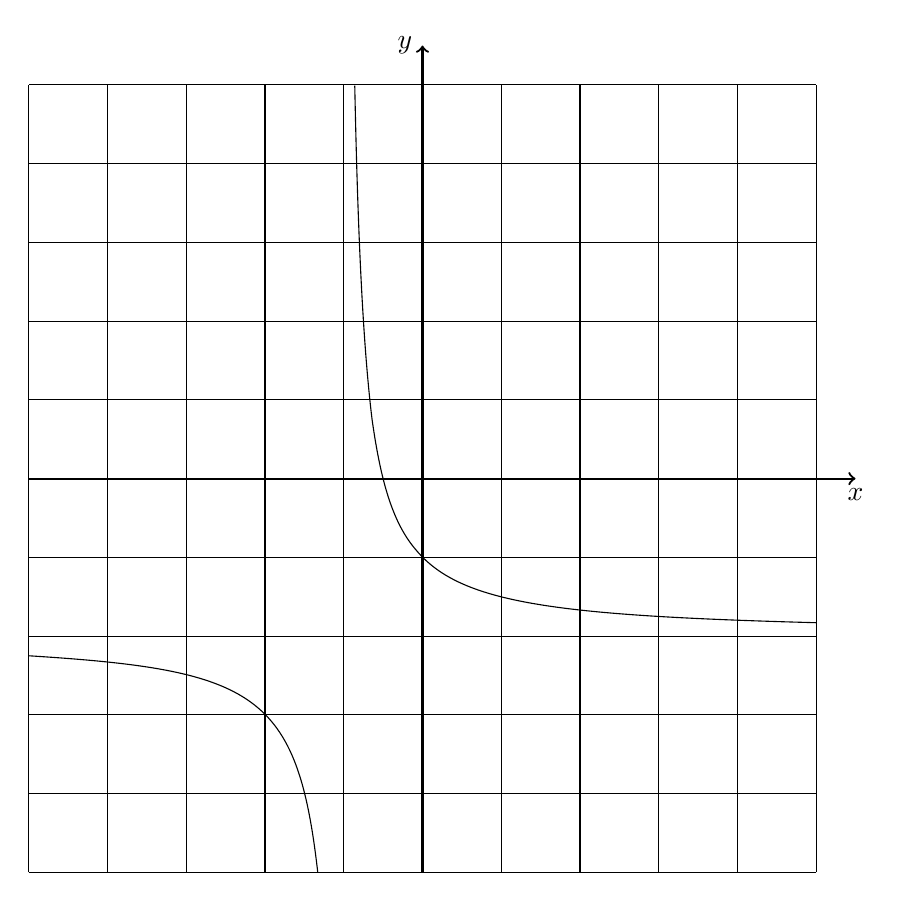
\begin{tikzpicture}
	\draw (-5,-5) grid (5,5);
	\draw[thick,->] (-5,0) -- (5.5,0) node[below]{$x$};
	\draw[thick,->] (0,-5) -- (0,5.5) node[left]{$y$};  
	\draw (-5,-2.25) .. controls (-2.12,-2.43) and (-1.59,-2.72) .. (-1.33,-5)
	(-0.86,4.99) .. controls (-0.82,3.01) and (-0.75,1.65) .. (-0.64,0.75) 
	.. controls (-0.53,-0.03) and (-0.38,-0.57) .. (-0.07,-0.92) 
	.. controls (0.5,-1.59) and (1.7,-1.74) .. (5,-1.83);
\end{tikzpicture}
\end{document}
\end{verbatim}
and you will get the following picture:
\begin{center}
	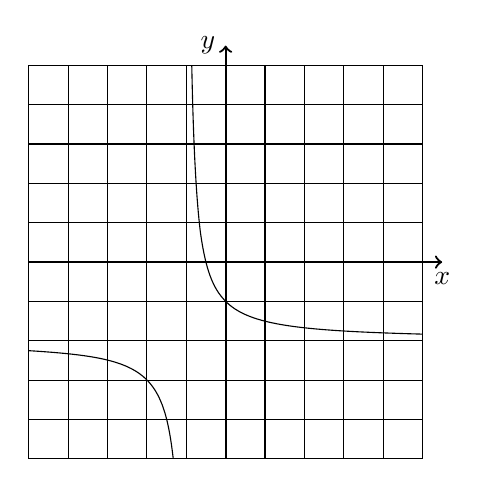
\begin{tikzpicture}[scale=.5]
		\draw (-5,-5) grid (5,5);
		\draw[thick,->] (-5,0) -- (5.5,0) node[below]{$x$};
		\draw[thick,->] (0,-5) -- (0,5.5) node[left]{$y$};  
		\draw (-5,-2.25) .. controls (-2.12,-2.43) and (-1.59,-2.72) .. (-1.33,-5)(-0.86,4.99) .. controls (-0.82,3.01) and (-0.75,1.65) 
	.. (-0.64,0.75) .. controls (-0.53,-0.03) and (-0.38,-0.57) .. (-0.07,-0.92) .. controls (0.5,-1.59) and (1.7,-1.74) .. (5,-1.83);
	\end{tikzpicture}
\end{center}
\section{Examples of \texttt{bezierplot} in Comparison with Gnuplot}
The following graphs are drawn with \texttt{bezierplot} (black) and Gnuplot (red). Gnuplot calculated 200 samples per example. The functions are given below the pictures (left: bezierplot, right: Gnuplot).
\begin{multicols}{3}
\graphcomparison{0.32*x-0.7}{0.32*x-0.7}
\graphcomparison{-x^2+4}{-x**2+4}
\graphcomparison{(x+1)*x*(x-1)}{(x+1)*x*(x-1)}
\graphcomparison{x^0.5}{x**0.5}
%\graphcomparison{x^(1/3)}{x**(1/3.)}
\graphcomparison{cbrt(x)}{sgn(x)*abs(x)**(1/3.)}
\graphcomparison{x^3*(x-1)}{x**3*(x-1)}
\graphcomparison{2*cos(3*x+4)+3}{2*cos(3*x+4)+3}
\graphcomparison{tan(x)}{tan(x)}
\graphcomparison{x+0.5*sin(x)}{x+0.5*sin(x)}
%\graphcomparison{1/(x-2)+1}{1/(x-2)+1}
\graphcomparison{2*x^2/(3*x-3)}{2*x**2/(3*x-3)}
\graphcomparison{4-exp(x)}{4-exp(x)}
\graphcomparison{log(x+4)}{log(x+4)}
\end{multicols}
\section{Are the Graphs Produced by bezierplot Exact?}
The graphs of quadratic and cubic functions and their inverse are exact (up to numeric precision). Parabola and sine and cosine functions use the predefined splines from Ti\emph{k}Z if possible. E.g.:
\begin{verbatim}
bezierplot "0.5*x^2-2*x-1"
\end{verbatim}
outputs
\begin{verbatim}
(-2,5) parabola bend (2,-3) (5,1.5)
\end{verbatim}
or
\begin{verbatim}
bezierplot "cos(x)"
\end{verbatim}
outputs
\begin{verbatim}
(-5,0.28) .. controls (-4.91,0.2) and (-4.82,0.11) .. (-4.71,0) 
sin (-3.14,-1) cos (-1.57,0) sin (0,1) cos (1.57,0) sin (3.14,-1) cos (4.71,0) 
.. controls (4.82,0.11) and (4.91,0.2) .. (5,0.28)
\end{verbatim}
\section{Options}
You can set the window of the graph as follows:
\begin{verbatim}
bezierplot "FUNCTION" XMIN XMAX YMIN YMAX
\end{verbatim}
e.g.
\begin{verbatim}
bezierplot "FUNCTION" 0 1 -3 2.5
\end{verbatim}
will set $0\leq x\leq 1$ and $-3\leq y\leq 2.5$. You may also omit the $y$--range, hence
\begin{verbatim}
bezierplot "FUNCTION" 0 1
\end{verbatim}
will set $0\leq x\leq 1$ and leave the default $-5\leq y\leq 5$.
\section{Daily Use with \LaTeX{} and Lua\LaTeX}
Supposing your OS finds \texttt{bezierplot} automatically (e.g. because it is in \verb|/usr/local/bin|), you can set up your \LaTeX{} file like this:
\begin{verbatim}
\documentclass{article}
\usepackage{tikz}
\makeatletter\let\evaluatedinput\@@input\makeatother
\providecommand{\bezierplot}[1]{\evaluatedinput|"bezierplot '#1'" }
\begin{document}
\tikz \draw \bezierplot{x^2};
\end{document}
\end{verbatim}
If you run \LaTeX{} with enabled shell-escape (option \verb|--shell-escape| for \TeX{}Live, option \verb|--write18| for MiK\TeX{}), you will receive automatically the following picture:
\begin{center}
	\begin{tikzpicture}[scale=.5]
		\draw (-2.24,5) parabola bend (0,0) (2.24,5);
	\end{tikzpicture}
\end{center}
Things get even better with Lua\LaTeX{}, because it can call Lua directly and do not need shell-escape enabled:
\begin{verbatim}
\documentclass{article}
\usepackage{tikz}
\directlua{require("bezierplot")}
\providecommand{\bezierplot}[1]{\directlua{tex.sprint(bezierplot("#1",-5,5,-5,5))}}
\begin{document}
\tikz \draw \bezierplot{x^2};
\end{document}
\end{verbatim}
Of course, you can improve the command \verb|\bezierplot| with optional arguments for the lower and upper bounds.
\end{document}
